\documentclass[12pt,a4paper]{extarticle}
\usepackage{../templates/preamble}

\renewcommand{\typeofnum}{1}
\renewcommand{\papertheme}{Представления строк.}

\begin{document}
\begin{titlepage}
    \begin{center}
        {\bfseries\large
        МИНОБРНАУКИ РОССИИ\par
        САНКТ-ПЕТЕРБУРГСКИЙ ГОСУДАРСТВЕННЫЙ\par
        ЭЛЕКТРОТЕХНИЧЕСКИЙ УНИВЕРСИТЕТ\par
        <<ЛЭТИ>> ИМ. В.И. УЛЬЯНОВА (ЛЕНИНА)\par
        Кафедра \department
        
        \vspace{0.23\textheight}
        
        \typeof
        по дисциплине <<\discipline>>\par
        Тема: \papertheme
        
        \vspace{0.28\textheight}
        }
        \begin{table}[h!]
            \centering\large
            \begin{tabularx}{\textwidth}{p{60mm}X>{\centering\arraybackslash}p{45mm}}
                Студент гр. 4352 & \_\_\_\_\_\_\_\_\_\_\_\_\_\_\_\_\_\_\_\_ & {Даричев Е. М.} \\ [5.4mm]  % Line height
                Преподаватель    & \_\_\_\_\_\_\_\_\_\_\_\_\_\_\_\_\_\_\_\_ & {\teacher} \\ [5.4mm]
            \end{tabularx}
        \end{table}

        \vspace{0.1\textheight}
        \large
        Санкт-Петербург\par
        \yyear
    \end{center}
\end{titlepage}

\setcounter{page}{2}
\tableofcontents
\newpage

% document %
\section{Исходная формулировка задания}
Преобразовать заданную строку следующим образом: каждую точку заменить многоточием. Реализовать
два варианта задания строк: с помощью разделителей и по количеству запрашиваемых символов.
Реализовать два представления строк: маркерный и по длине.

\section{Определение неясностей}
Разделитель определяет конец строки, сохраняемой в памяти. Маркер конца строки обозначает конец
интересующей строки, текст после маркера не влияет на результирующую строку. В качестве этих символов
могут выступать любые символы таблицы ASCII.

При использовании динамического выделения памяти второй вариант ввода сводится к тому, что
количество запрашиваемых символов всегда равно длине строки. В таком случае для обработки будет забираться
вся строка.

\section{Контрольный пример}
Ниже приведены контрольные примеры маркерного представления, в которых в качестве разделителя
принят символ <<*>>, а в качестве маркера --- <<@>>.

\begin{table}[h]
    \centering
    \begin{tabularx}{\textwidth}{|t|t|}
        \hline
        \multicolumn{1}{|h|}{Ввод} & \multicolumn{1}{h|}{Вывод} \\ \hline
        Строка с точками. И ограничит*елем & Строка с точками... И ограничит@ \\ \hline
        Много..точек...подряд & Много......точек.........подряд@ \\ \hline
        Несколько ограничителей*** & Несколько ограничителей@ \\ \hline
        Маркер.перед.огр@аничителем* & Маркер...перед...огр@ \\ \hline
        Др!!угие."сим"волы\$\$\#*??* & Др!!угие..."сим"волы\$\$\#@ \\ \hline
    \end{tabularx}
\end{table}

Ниже приведены примеры представления по длине, в которых в качестве разделителя принят символ <<@>>.

\begin{table}[h!]
    \centering
    \begin{tabularx}{\textwidth}{|t|t|}
        \hline
        \multicolumn{1}{|h|}{Ввод}         & \multicolumn{1}{h|}{Вывод} \\ \hline
        Строка. И ограничит*елем           & Строка... И ограничит*елем \\ \hline
        Много..точек...подряд              & Много......точек.........подряд \\ \hline
        Несколько ограничителей@@@         & Несколько ограничителей \\ \hline
        Маркер.перед.огр@аничителем*       & Маркер...перед...огр \\ \hline
        Др!!угие."сим"волы\$\$\#*??*       & Др!!угие..."сим"волы\$\$\#*??* \\ \hline
    \end{tabularx}
\end{table}

\section{Ограничения, обусловленные вычислительным устройством}
Ограничения могут накладываться на максимальное количество памяти,
которое можно выделить для динамического массива символов.

\section{Организация интерфейса пользователя}
Интерфейс реализован шаблонами:

O1 (приветственное сообщение и запрос версии ввода):\\
{\ttfamily\footnotesize
Задание: Преобразовать заданную строку следующим образом: каждую точку

заменить многоточием

Даричев Егор а.г. 4352

Введите номер варианта ввода: [I1]
}

I1 (запрос версии файла): {\ttfamily\footnotesize \{1|2\}}

O2/3: {\ttfamily\footnotesize Не удалось открыть файл ввода/вывода}

O4: {\ttfamily\footnotesize Неверный номер варианта}

O5: {\ttfamily\footnotesize Вывод результата в консоль и выходной файл:\par
[формат выходного файла]}

\section{Формат файлов}
Входные и выходные файлы для маркерного представления должны иметь следующие форматы:
\newpage

\begin{xltabular}{\textwidth}{|t|t|}
    \hline
    \multicolumn{2}{|>{\centering\arraybackslash}X|}{Входные файлы} \\ \hline
    \multicolumn{1}{|h|}{Вариант 1} & \multicolumn{1}{h|}{Вариант 2} \\ \hline
    RM \normalfont //символы разделителя и маркера\par\ttfamily
    [c...]\{R|M|\}[c...] \normalfont //первая строка\par\ttfamily
    [c...]\{R|M|\}[c...] \normalfont //вторая строка\par\ttfamily
    ... &
    M \normalfont //символ маркера\par\ttfamily
    [c...]\{M|\}[c...] \normalfont //первая строка\par\ttfamily
    [c...]\{M|\}[c...] \normalfont //вторая строка\par\ttfamily
    ... \\ \hline

    \multicolumn{2}{|>{\centering\arraybackslash}X|}{Выходные файлы} \\ \hline
    \multicolumn{2}{|t|}{
    [c...]M \normalfont //первая строка\par\ttfamily
    [c...]M \normalfont //вторая строка\par\ttfamily
    ...
    } \\ \hline
\end{xltabular}

Входные и выходные файлы для представления по длине должны иметь следующие форматы:

\begin{xltabular}{\textwidth}{|t|t|}
    \hline
    \multicolumn{2}{|>{\centering\arraybackslash}X|}{Входные файлы} \\ \hline
    \multicolumn{1}{|h|}{Вариант 1} & \multicolumn{1}{h|}{Вариант 2} \\ \hline
    R \normalfont //символы разделителя и маркера\par\ttfamily
    [c...]\{R|\}[c...] \normalfont //первая строка\par\ttfamily
    [c...]\{R|\}[c...] \normalfont //вторая строка\par\ttfamily
    ... &
    [c...] \normalfont //первая строка\par\ttfamily
    [c...] \normalfont //вторая строка\par\ttfamily
    ... \\ \hline

    \multicolumn{2}{|>{\centering\arraybackslash}X|}{Выходные файлы} \\ \hline
    \multicolumn{2}{|t|}{
    [c...] \normalfont //первая строка\par\ttfamily
    [c...] \normalfont //вторая строка\par\ttfamily
    ...
    } \\ \hline
\end{xltabular}

\section{Реализация ввода/вывода}
\begin{xltabular}{\textwidth}{|h|s|s|}
    \hline
    \multicolumn{1}{|h|}{Библиотека} &
    \multicolumn{1}{s|}{Ввод} &
    \multicolumn{1}{s|}{Вывод}\\ \hline
    iostream & cin > > & cout < < \\ \hline
\end{xltabular}

\section{Внутреннее представление данных}
\begin{xltabular}{\textwidth}{|
>{\hsize=.2\hsize\centering\arraybackslash\ttfamily\bfseries}X|
>{\hsize=.1\hsize\centering\arraybackslash\itshape}X|
>{\hsize=.7\hsize\centering\arraybackslash}X|
}
\hline
\multicolumn{1}{|>{\hsize=.2\hsize\centering\arraybackslash}X}{Имя переменной} &
\multicolumn{1}{|>{\hsize=.1\hsize\centering\arraybackslash}X}{Тип} &
\multicolumn{1}{|>{\hsize=.7\hsize\centering\arraybackslash}X|}{Описание} \\ \hline
ifstream & in & Входной файл \\ \hline
ofstream & out & Выходной файл \\ \hline
strings & str* | StringLen* & Массив считанных строк \\ \hline    
\end{xltabular}
Структура {\ttfamily\bfseries str}:
\begin{xltabular}{\textwidth}{|
>{\hsize=.2\hsize\centering\arraybackslash\ttfamily\bfseries}X|
>{\hsize=.1\hsize\centering\arraybackslash\itshape}X|
>{\hsize=.7\hsize\centering\arraybackslash}X|
}
\hline
\multicolumn{1}{|>{\hsize=.2\hsize\centering\arraybackslash}X}{Имя аргумента} &
\multicolumn{1}{|>{\hsize=.1\hsize\centering\arraybackslash}X}{Тип} &
\multicolumn{1}{|>{\hsize=.7\hsize\centering\arraybackslash}X|}{Описание} \\ \hline
symbols & char* & Символы строки \\ \hline
mark & char & Символ-маркер \\ \hline
ellipsis\_\par length & unsigned & Длина вставляемого многоточия \\ \hline    
\end{xltabular}

Класс {\ttfamily\bfseries StringLen}:
\begin{xltabular}{\textwidth}{|
>{\hsize=.2\hsize\centering\arraybackslash\ttfamily\bfseries}X|
>{\hsize=.1\hsize\centering\arraybackslash\itshape}X|
>{\hsize=.7\hsize\centering\arraybackslash}X|}
\hline
\multicolumn{1}{|>{\hsize=.2\hsize\centering\arraybackslash}X}{Имя аргумента} &
\multicolumn{1}{|>{\hsize=.1\hsize\centering\arraybackslash}X}{Тип} &
\multicolumn{1}{|>{\hsize=.7\hsize\centering\arraybackslash}X|}{Описание} \\ \hline
\_text & char* & Символы строки \\ \hline
\_len & unsigned & Длина строки \\ \hline
\end{xltabular}

\section{Описание функций}
\subsection{Параметры}
\begin{xltabular}
    {\textwidth}{|X|X|X|X|X|X|}
    \hline
    \multirow{2}{0.14\textwidth}{\centering Имя функции} &
    \multicolumn{4}{c|}{Параметры} &
    \multirow{2}{0.14\textwidth}{\centering Возращаемый тип} \\ \cline{2-5}
    & Входные & Выходные & Модифицир. & Транзитные & \\ \hline
    str::next & unsigned i & & & & bool \\ \hline
    str::process &&&&& void \\ \hline
    str::print\_to & ostream \&out && ostream \&out && void \\ \hline
    str::put & char ch, unsigned *at && unsigned *at & unsigned *at & void \\ \hline
    input1 & istream \&in, unsigned *v & unsigned *v & istream \&in & unsigned *v & str* \\ \hline
    input2 & istream \&in, unsigned *v & unsigned *v & istream \&in & unsigned *v & str* \\ \hline
    StringLen::\newline process &&&&& void \\ \hline
    StringLen::print & ostream \&out && ostream \&out && void \\ \hline
    input & istream \&in, unsigned *v & unsigned *v & istream \&in & unsigned *v & StringLen* \\ \hline
\end{xltabular}

\subsection{Функции}
\subsubsection{Структура str}
\begin{listed}
    \item str::next \newline
    Принимает текущий индекс и определяет, можно ли продолжать проходить по строке.
    \item str::process \newline
    Основная функция, выполняющая задание.
    \item str::print\_to \newline
    Принимает выходной поток и выводит в него строку, включая маркер.
    \item str::put \newline
    Принимает символ и длину текущей строки, ставит символ в конец.
    \item input1/input2 \newline
    Ввод. Принимает входной поток и ссылку на переменную, указывающую на количество считанных
    строк.
\end{listed}

\subsubsection{Класс StringLen}
\begin{listed}
    \item StringLen::StringLen \newline
    Конструкторы, без аргументов инициализирует пустой объект, иначе принимает указатель на строку и длину строки.
    Если аргумент --- объект этого класса, то он копируется.
    \item StringLen::~StringLen \newline
    Деструктор, освобождает память, которую занимает строка.
    \item StringLen::StringLen\& operator= \newline
    Оператор приравнивания. Используется, чтобы поменять местами значения двух объектов.
    \item StringLen::process \newline
    Выполняет задание ня текущей строке.
    \item StringLen::print \newline
    Принимает поток и выводит в него строку.
    \item input \newline
    Две версии ввода. Обе принимают входной поток и ссылку на переменную, указывающую на количество считанных
    строк.
\end{listed}

\section{Описание алгоритма}
Алгоритм обработки строки сводится к подсчёту количества точек в строке, проходясь по ней, пока не встретим
маркер. Далее выделяется память по формуле $1 + i + dots\_count\cdot(ellipsis\_length - 1)$, где $i$ --- инкремент
предыдущей операции. После этого выполняется проход по исходной строке и посимвольный перенос в новую память, пока
не встретится точка. Если встречается точка, проход останавливается, а в новую память записывается $ellipsis\_length$
точек подряд.

{\centering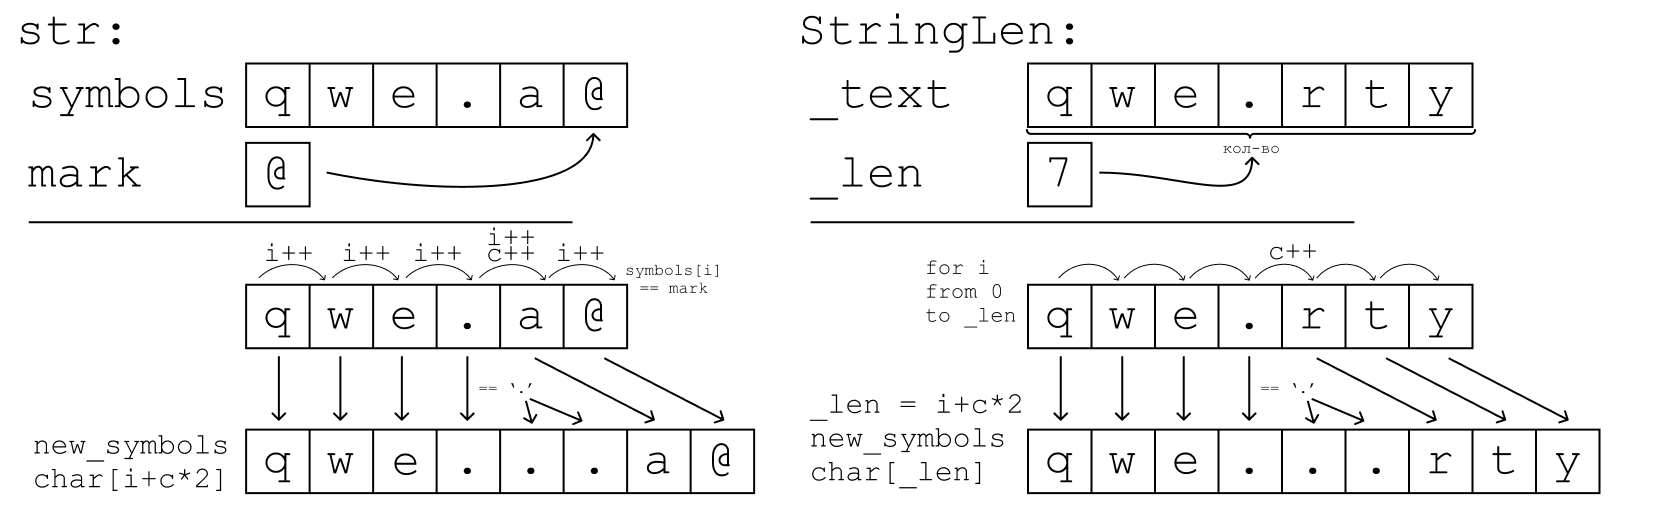
\includegraphics[width=\linewidth]{figures/Frame 11.png}}

Ниже представлены блок-схемы функций.
\begin{center}
    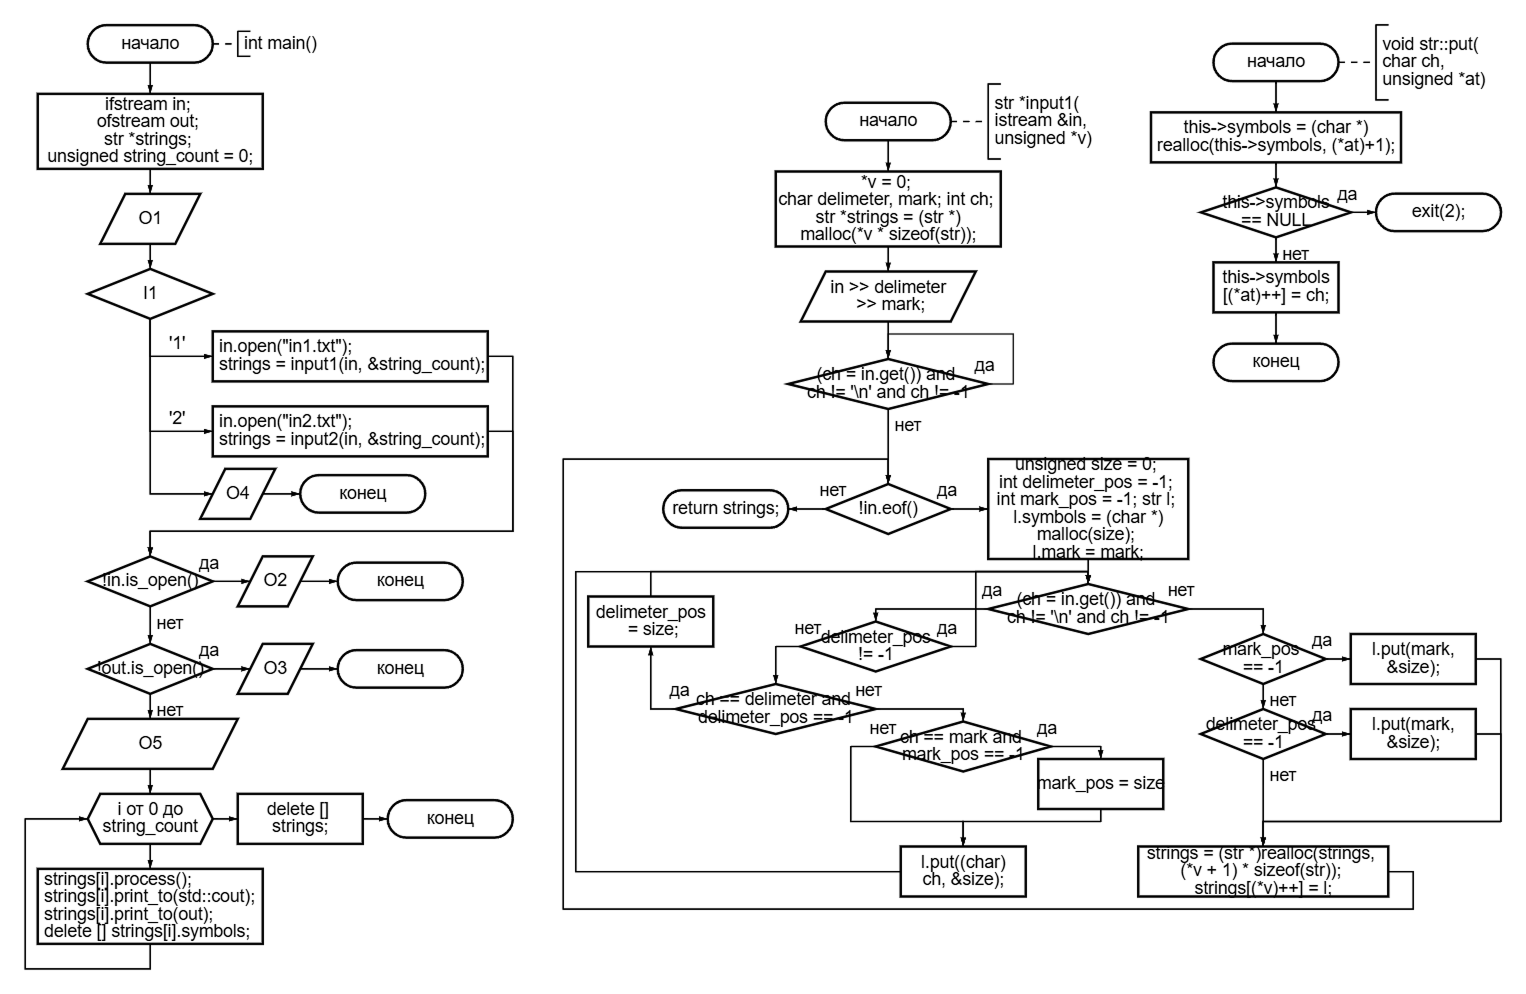
\includegraphics[width=\linewidth]{figures/Frame 3.png}
    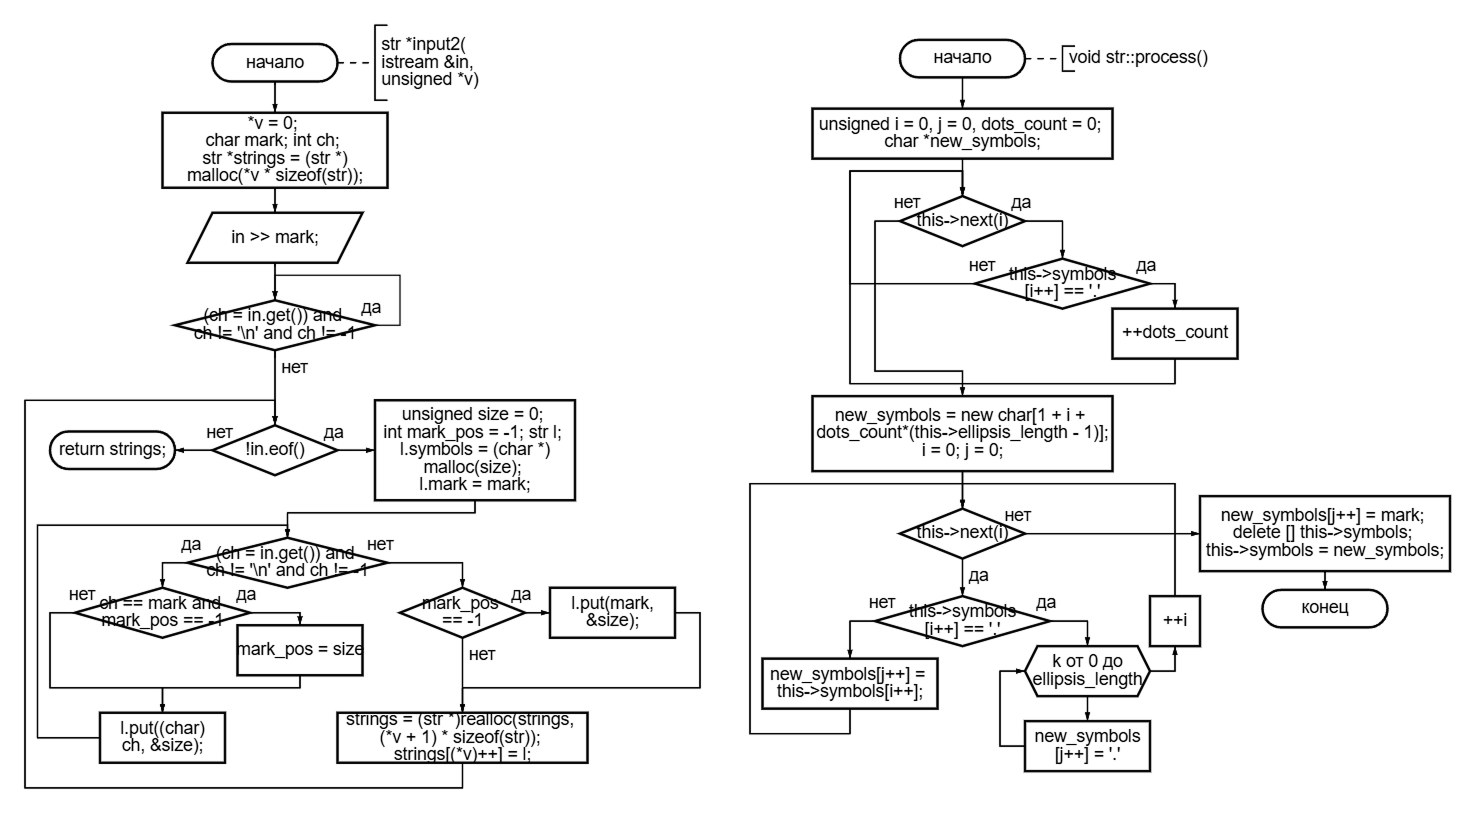
\includegraphics[width=\linewidth]{figures/Frame 4.png}
    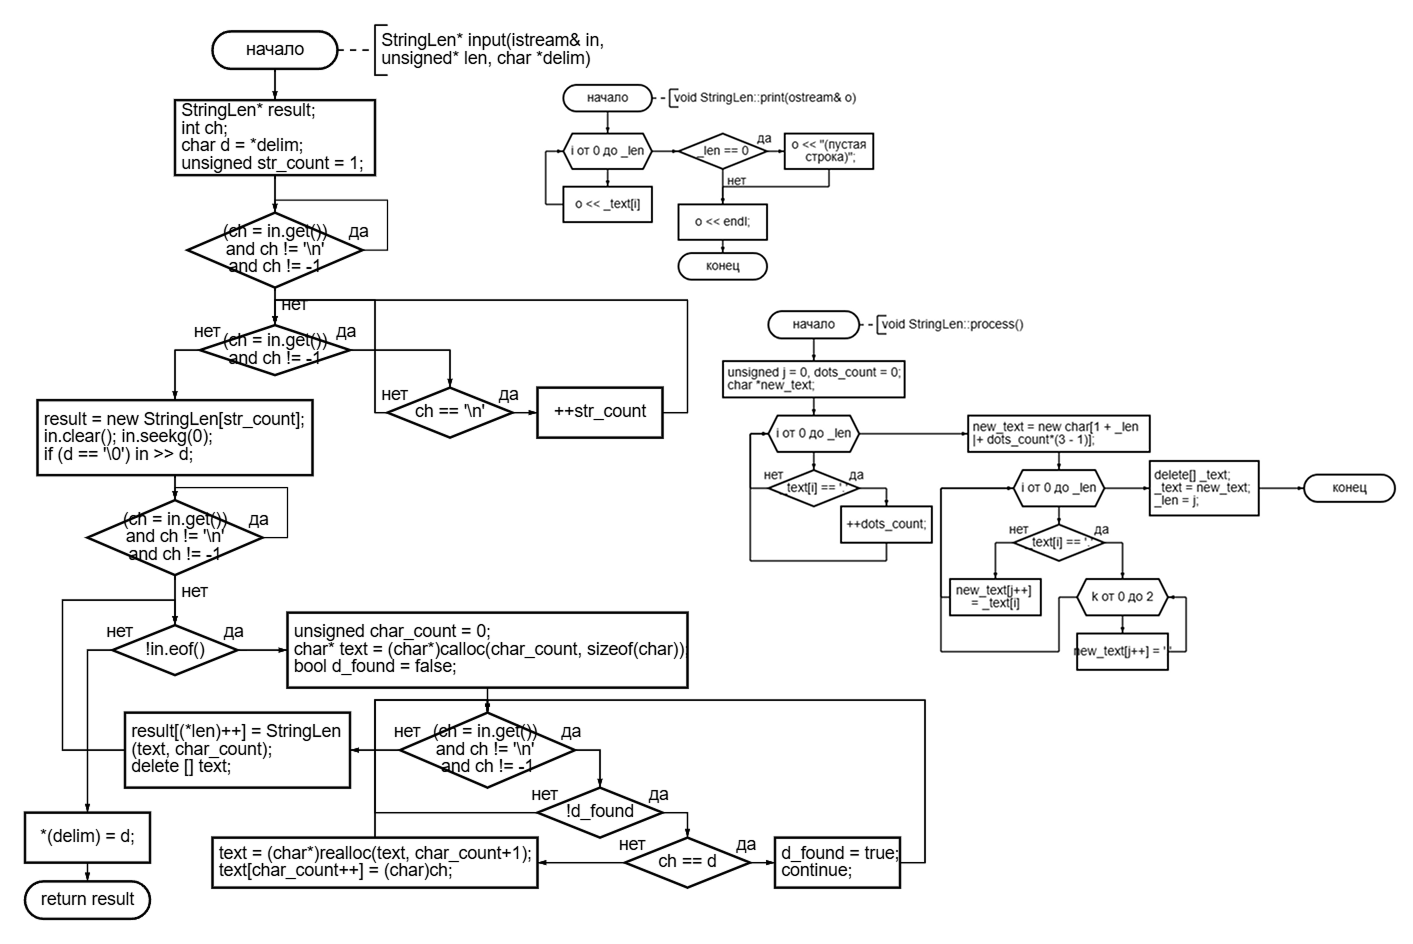
\includegraphics[width=\linewidth]{figures/Frame 5.png}
\end{center}

\section{Исходный код программы}

Код программы маркерного представления:
\lstinputlisting[language=C++]{../../tasks/1.1/main.cpp}

Код программы представления по длине:
\lstinputlisting[language=C++]{../../tasks/1.2/main.cpp}

\newpage
\section{Результаты работы программы}
\subsection{Маркерное представление}
\begin{xltabular}
    {\linewidth}{|H|H|} \hline
    \multicolumn{1}{|h}{Вход 1} & \multicolumn{1}{|h|}{Вход 2} \\ \hline
    \multicolumn{2}{|X|}{\lstinputlisting{../../tasks/1.1/in.txt}} \\ \hline
    \multicolumn{1}{|h}{Выход 1} & \multicolumn{1}{|h|}{Выход 2} \\ \hline
    ... & ... \\ \hline
\end{xltabular}

\subsection{Представление по длине}

\section{Вывод о проделанной работе}
В ходе выполнения работы я научился такой структуре данных, как маркированная строка, как работать с ней, распределяя память динамически.

\end{document}
